\documentclass[a4paper]{article}
\usepackage{amsfonts}
\usepackage{amsmath}
\addtolength{\hoffset}{-2.25cm}
\addtolength{\textwidth}{4.5cm}
\addtolength{\voffset}{-3.25cm}
\addtolength{\textheight}{5cm}
\setlength{\parindent}{15pt}

\usepackage[unicode=true, colorlinks=false, hidelinks]{hyperref}
\usepackage[utf8]{inputenc}
\usepackage[english, russian]{babel}
\usepackage{mathtext}
\usepackage[T2A, TS1]{fontenc}
\usepackage{microtype} % Slightly tweak font spacing for aesthetics
\usepackage{amsthm, amssymb, amsmath, amsfonts, nccmath}
\usepackage{nicefrac}
\usepackage{epstopdf}
\usepackage[export]{adjustbox}
\usepackage{float} % Improved interface for floating objects
\usepackage{graphicx, multicol} % Enhanced support for graphics
\usepackage{pdfrender,xcolor}
\usepackage{breqn}
\usepackage{mathtools}
\usepackage{titling}
\usepackage{bm}
\usepackage{centernot}
\usepackage[cal=boondoxo,calscaled=.96]{mathalpha}
\usepackage{marvosym, wasysym} % More symbols
\usepackage{rotating} % Rotation tools
\usepackage{censor} % Facilities for controlling restricted text

\usepackage{fancyhdr}
\pagestyle{fancy}
\fancyhead{}\renewcommand{\headrulewidth}{0pt}
\fancyfoot[L]{}
\fancyhead{}
\fancyfoot{}
\fancyfoot[R]{\thepage}
\begin{document}
    \begin{titlepage}
   \begin{center}
       \vspace*{3cm}
       \large{САНКТ-ПЕТЕРБУРГСКИЙ ПОЛИТЕХНИЧЕСКИЙ УНИВЕРСИТЕТ}
       \vspace{0.4 cm}

       \large\textbf{Институт прикладной математики и механики}
       \vspace{0.4 cm}

       \large{Высшая школа прикладной математики и вычислительной физики}

       \vspace{3 cm}
       \normalsize\textbf{Отчет\\ по лабораторной работе №7\\ по дисциплине\\
«Математическая статистика»}
       \vfill
       \begin{flushright}
            \normalsize{Выполнил студент:\\
            Антонов Алексей\\
            группа: 3630102/80201}
            \vskip\medskipamount
            \normalsize{Проверил:

            к.ф.-м.н., доцент\\
            Баженов Александр Николаевич
            }
       \end{flushright}

       \vspace{0.8cm}


       \normalsize{Санкт-Петербург\\2021 г.}

   \end{center}
\end{titlepage}
    \tableofcontents
    \newpage
	\listoffigures
    \newpage
	\listoftables
    \newpage
\section {Постановка задачи}
	Для 5 распределений:
    \begin{itemize}
        \item Нормальное распределение $N(x, 0, 1)$
        \item Распределение Коши $C(x, 0, 1)$
        \item Распределение Лапласа $L\left(x, 0, \frac{1}{\sqrt{2}}\right)$
        \item Распределение Пуассона $P(k, 10)$
        \item Равномерное распределение $U\left(x,-\sqrt{3},\sqrt{3}\right)$
    \end{itemize}
	\begin{enumerate}
    	\item Сгенерировать выборки размером 10, 50 и 1000 элементов. Построить на одном рисунке гистограмму и график плотности распределения.
    	\item Сгенерировать выборки размером 10, 100 и 1000 элементов.
    	Для каждой выборки вычислить следующие статистические характеристики положения данных: $\overline{x}, med\,x, z_R, z_Q, z_{tr}$. Повторить такие вычисления 1000 раз для каждой выборки и найти среднее характеристик положения и их квадратов:
    	\begin{equation}\label{mean_formula}
        	E(z)=\overline{z}
    	\end{equation}
    	Вычислить оценку дисперсии по формуле:
    	\begin{equation}\label{variance_formula}
        	D(z)=\overline{z^2}-\overline{z}^2
    	\end{equation}
    	Представить полученные данные в виде таблиц.
		\item Сгенерировать выборки размером 20 и 100 элементов. Построить для них боксплот Тьюки. Для каждого распределения определить долю выбросов экспериментально (сгенерировав выборку, соответствующую распределению 1000 раз, и вычислив среднюю долю выбросов) и сравнить с результатами, полученными теоретически.
		\item Сгенерировать выборки размером 20, 60 и 100 элементов. Построить на них эмпирические функции распределения и ядерные оценки плотности распределения на отрезке $[-4;\,4]$ для непрерывных распределений и на отрезке $[6;\,14]$ для распределения Пуассона.
	\end{enumerate}

\section {Теория}
	\subsection{Рассматриваемые распределения}
    Плотности:
    \begin{itemize}
        \item Нормальное распределение
        \begin{equation}\label{eq:norm}
            N(x,0,1)=\frac{1}{\sqrt{2\pi}}e^{-\frac{x^2}{2}}
        \end{equation}
        \item Распределение Коши
        \begin{equation}\label{eq:cauchy}
            C(x, 0, 1)=\frac{1}{\pi}\frac{1}{x^2+1}
        \end{equation}
        \item Распределение Лапласа
        \begin{equation}\label{eq:laplace}
            L(x,0,\frac{1}{\sqrt{2}})=\frac{1}{\sqrt{2}}e^{-\sqrt{2}|x|}
        \end{equation}
        \item Распределение Пуассона
        \begin{equation}\label{eq:poisson}
            P(k, 10)=\frac{10^k}{k!}e^{-10}
        \end{equation}
        \item Равномерное распределение
            \begin{equation}\label{eq:uniform}
                U(x,-\sqrt{3},\sqrt{3})=
                \begin{cases}
                \displaystyle\frac{1}{2\sqrt{3}}&\text{при}\;\;|x|\:\leq\sqrt{3}\\
                \;\;\;0&\text{при}\;\;|x|\:>\sqrt{3}\\
                \end{cases}
            \end{equation}
		\end{itemize}
	\subsection{Гистограмма}
		\subsubsection{Построение гистограммы}
		Множество значений, которое может принимать элемент выборки, разбивается на несколько одинаковых интервалов, откладываемых на горизонтальной оси, над каждым из которых затем рисуется прямоугольник.
		Высота каждого прямоугольника пропорциональна числу элементов выборки, попадающих в соответствующий интервал.


	\subsection{Вариационный ряд}
Последовательность $\displaystyle\{x_{(k)}\}_{k=1}^n$ элементов выборки размера $n$, расположенных в неубывающем порядке, называется вариационным рядом.
\subsection{Выборочные числовые характеристики}
\subsubsection{Характеристики положения}
\begin{itemize}
    \item Выборочное среднее
    \begin{equation}\label{mean}
        \overline{x}=\frac{1}{n}\sum_{i=1}^n x_i
    \end{equation}
    \item Выборочная медиана
    \begin{equation}\label{med}
        med\,x = \begin{cases}
        \displaystyle\;\;\;\;\;x_{(l+1)}&\text{при}\;\;n=2l+1\\
        \displaystyle\frac{x_{(l)}+x_{(l+1)}}{2}&\text{при}\;\;n=2l
        \end{cases}
    \end{equation}
    \item Полусумма экстремальных выборочных элементов
    \begin{equation}\label{exhfsum}
        z_R=\frac{x_{(1)}+x_{(n)}}{2}
    \end{equation}
    \item Полусумма квартилей\\
    Выборочный квартиль $z_p$ порядка $p$ определяется формулой
    \begin{equation}
        z_p = \begin{cases}\label{pqv}
        \displaystyle\;\;x_{([np]+1)}&\text{при}\;\;np\;\text{дробном,}\\
        \displaystyle\;\;\;\;\;x_{(np)}&\text{при}\;\;np\;\text{целом}
        \end{cases}
    \end{equation}
    Полусумма квартилей
    \begin{equation}\label{eq:hfsum}
        z_Q=\frac{z_{1/4}+z_{3/4}}{2}
    \end{equation}
    \item Усечённое среднее
    \begin{equation}\label{eq:trmean}
        z_{tr}=\frac{1}{n-2r}\sum_{i=r+1}^{n-r}x_{(i)},\;\;r\approx\frac{n}{4}
    \end{equation}
\end{itemize}
    \subsubsection{Характеристики рассеивания}
Выборочная дисперсия
\begin{equation}\label{eq:svar}
    D=\frac{1}{n}\sum_{i=1}^n \left(x_i-\overline{x}\right)^2
\end{equation}

	\subsection{Боксплот Тьюки}
	\subsubsection{Определение}
	\noindent Боксплот (англ. box plot) — график, использующийся в описательной статистике, компактно изображающий одномерное распределение вероятностей

	\subsubsection{Описание}
	\noindent Такой вид диаграммы в удобной форме показывает медиану, нижний и верхний квартили и выбросы. Несколько таких ящиков можно нарисовать бок о бок, чтобы визуально сравнивать одно распределение с другим; их можно располагать как горизонтально, так и вертикально. Расстояния между различными частями ящика позволяют определить степень разброса (дисперсии) и асимметрии данных и выявить выбросы.

	\subsubsection{Построение}
	\noindent Границами ящика служат первый и третий квартили, линия в середине ящика — медиана. Концы усов — края статистически значимой выборки (без выбросов). Длину «усов» определяют разность первого квартиля и полутора межквартильных расстояний и сумма третьего квартиля и полутора межквартильных расстояний. Формула имеет вид
	\begin{equation}
	\label{mouns}
	{X_1 = Q_1-} \frac{3}{2}{(Q_3 - Q_1)},   {X_2 = Q_3+} \frac{3}{2}{(Q_3 - Q_1)}
	\end{equation}
	где $X_1$ — нижняя граница уса, $X_2$ — верхняя граница уса, $Q_1$ — первый квартиль, $Q_3$ — третий квартиль. Данные, выходящие за границы усов (выбросы), отображаются на графике в виде маленьких кружков.


\subsection{Теоретическая вероятность выбросов}
	\noindent Встроенными средствами языка программирования Python в среде разработки PyCharm можно вычислить теоретические первый и третий квартили распределений ($Q_1^T$ и $Q_3^T$ соответственно). По формуле \eqref{mouns} можно вычислить теоретические нижнюю и верхнюю границы уса ($X_1^T$ и $X_2^T$ соответственно). Выбросами считаются величины x, такие что:
	\begin{equation}
		\left[
		\begin{gathered}
		x < X_1^T \\
		x > X_2^T \\
		\end{gathered}
		\right.
	\end{equation}
	Теоретическая вероятность выбросов для непрерывных распределений
	\begin{equation}
		P_B^T = P(x<X_1^T) + P(x>X_2^T)=F(X_1^T) + (1-F(X_2^T))
	\end{equation}
	где $F(X)=P(x\leq{X})$ - функция распределения.
	Теоретическая вероятность выбросов для дискретных распределений
	\begin{equation}
		P_B^T = P(x<X_1^T)+P(x>x_2^T)=(F(X_1^T)-P(x=X_1^T))+(1-F(X_2^T))
	\end{equation}
	где $F(X) = P(x\leq{X})$ - функция распределения



	\subsection{Эмпирическая функция распределения}
		\subsubsection{Статистический ряд}
			\noindent Статистическим рядом назовем совокупность, состоящую из последовательности $\displaystyle\{z_i\}_{i=1}^k$ попарно различных элементов выборки, расположенных по возрастанию, и последовательности $\displaystyle\{n_i\}_{i=1}^k$ частот, с которыми эти элементы содержатся в выборке.
		\subsubsection{Эмпирическая функция распределения}
			\noindent Эмпирическая функция распределения (э. ф. р.) - относительная частота события $X < x$, полученная по данной выборке:
			\begin{equation}
				F_n^*(x)=P^*(X<x).
			\end{equation}
			\subsubsection{Нахождение э. ф. р.}
			\begin{equation}
				F^*(x)=\frac{1}{n}\sum_{z_i<x}n_i.
			\end{equation}
			$F^*(x)-$ функция распределения дискретной случайной величины $X^*$, заданной таблицей распределения
			\begin{table}[H]
				\centering
				\begin{tabular}{|c|c|c|c|c|}
					\hline
					 $X^*$&$z_1$&$z_2$&...&$z_k$\\
					 \hline
					 $P$&$n_1/n$&$n_2/n$&...&$n_k/n$\\
					 \hline
				\end{tabular}
				\caption{Таблица распределения}
				\label{tab:my_label}
			\end{table}
			\noindent Эмпирическая функция распределения является оценкой, т. е. приближённым значением, генеральной функции распределения
			\begin{equation}
				F_n^*(x)\approx F_X(x).
			\end{equation}
	\subsection{Оценки плотности вероятности}
		\subsubsection{Определение}
			\noindent Оценкой плотности вероятности $f(x)$ называется функция $\widehat{f}(x)$, построенная на основе выборки, приближённо равная $f(x)$
			\begin{equation}
				\widehat{f}(x)\approx f(x).
			\end{equation}
		\subsubsection{Ядерные оценки}
			\noindent Представим оценку в виде суммы с числом слагаемых, равным объёму выборки:
			\begin{equation}
				\widehat{f}_n(x)=\frac{1}{n h_n}\sum_{i=1}^n K\left(\frac{x-x_i}{h_n}\right).
			\end{equation}
			$K(u)$ - ядро, т. е. непрерывная функция, являющаяся плотностью вероятности, $x_1,...,x_n$ $-$ элементы выборки, а $\{h_n\}_{n\in\mathbb{N}}$ - последовательность элементов из $\mathbb{R}_+$ такая, что
			\begin{equation}
				h_n\xrightarrow[n\to\infty]{}0;\;\;\;n h_n\xrightarrow[n\to\infty]{}\infty.
			\end{equation}
			Такие оценки называются непрерывными ядерными.\\\\
			Гауссово ядро:
			\begin{equation}
				K(u)=\frac{1}{\sqrt{2\pi}}e^{-\frac{u^2}{2}}.
			\end{equation}
			Правило Сильвермана:
			\begin{equation}
				h_n=\left(\frac{4\hat{\sigma}^5}{3n}\right)^{1/5}\approx1.06\hat{\sigma}n^{-1/5},
			\end{equation}
			где $\hat{\sigma}$ - выборочное стандартное отклонение.
\section{Программная реализация}
Лабораторная работа выполнена на языке Python в среде PyCharm с использованием следующих библиотек:
\begin{enumerate}
    \item numpy
    \item scipy
    \item matplotlib
\end{enumerate}


\section {Результаты}
	\subsection{Гистограмма и график плотности распределения}
	\begin{figure}[H]
            \centering
            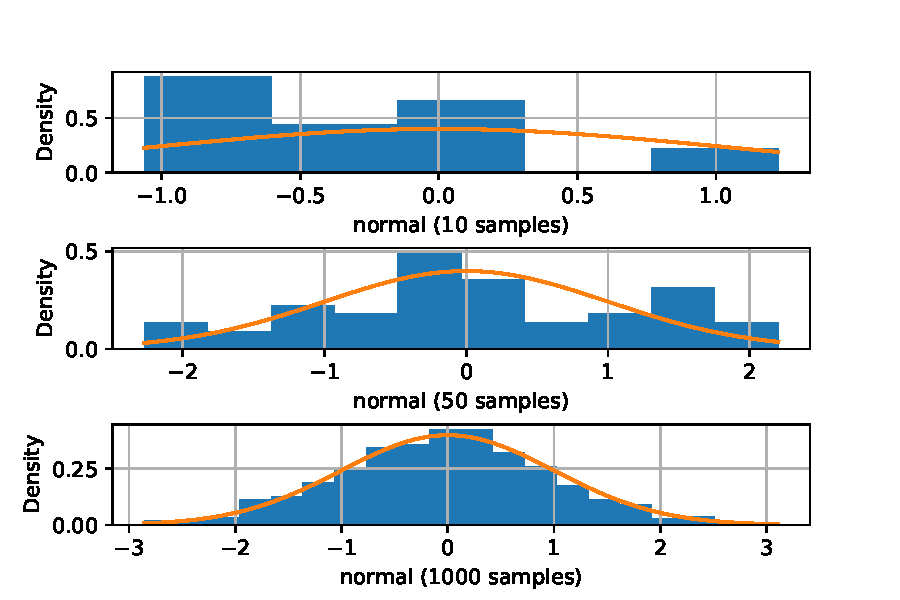
\includegraphics[width = 16 cm]{src_lab_1/normal}
            \caption{Нормальное распределение~\eqref{eq:norm}}
            \label{fig:norm}
        \end{figure}

        \begin{figure}[H]
            \centering
            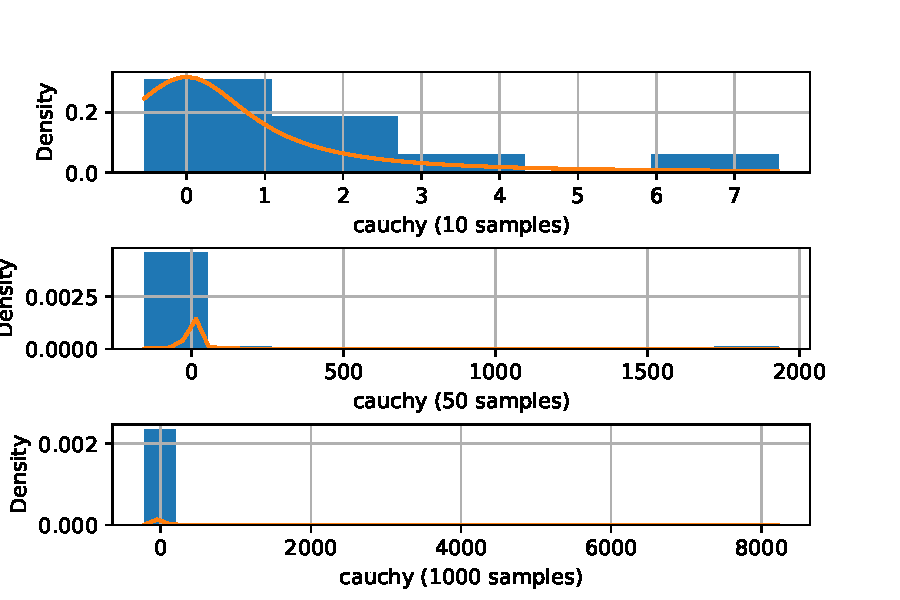
\includegraphics[width = 16 cm]{src_lab_1/cauchy}
            \caption{Распределение Коши~\eqref{eq:cauchy}}
            \label{fig:cauchy}
        \end{figure}

        \begin{figure}[H]
            \centering
            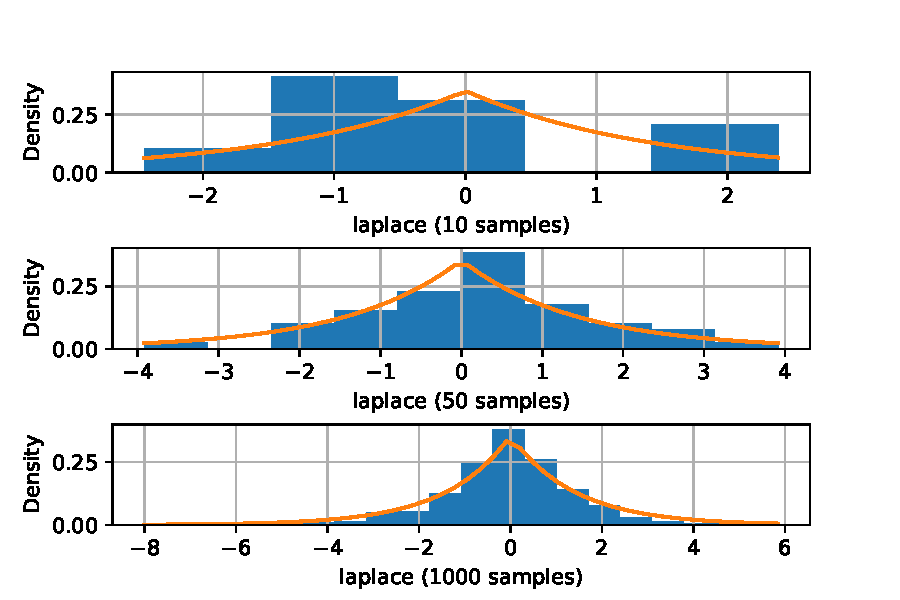
\includegraphics[width = 16 cm]{src_lab_1/laplace}
            \caption{Распределение Лапласа~\eqref{eq:laplace}}
            \label{fig:laplace}
        \end{figure}

        \begin{figure}[H]
            \centering
            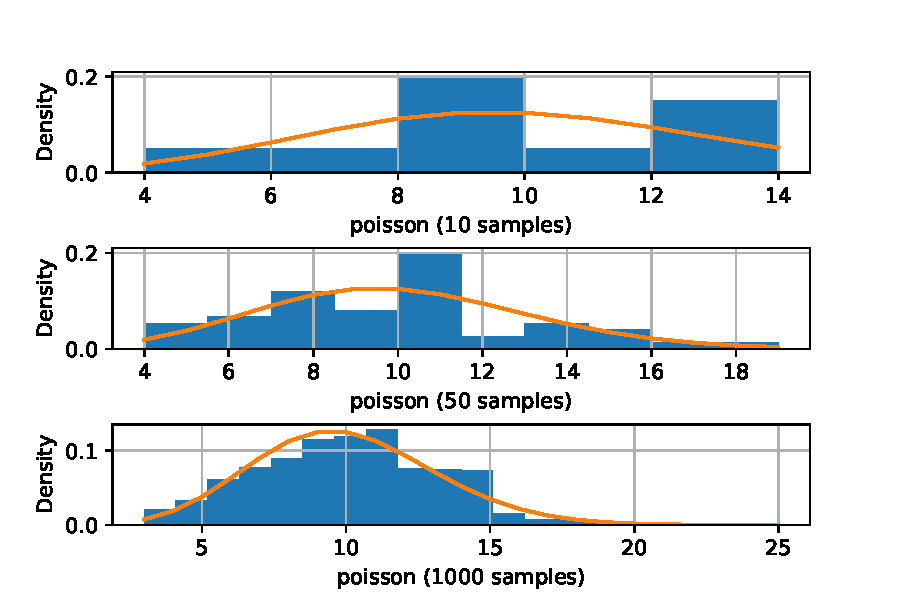
\includegraphics[width = 16 cm]{src_lab_1/poisson}
            \caption{Распределение Пуассона~\eqref{eq:poisson}}
            \label{fig:poisson}
        \end{figure}

        \begin{figure}[H]
            \centering
            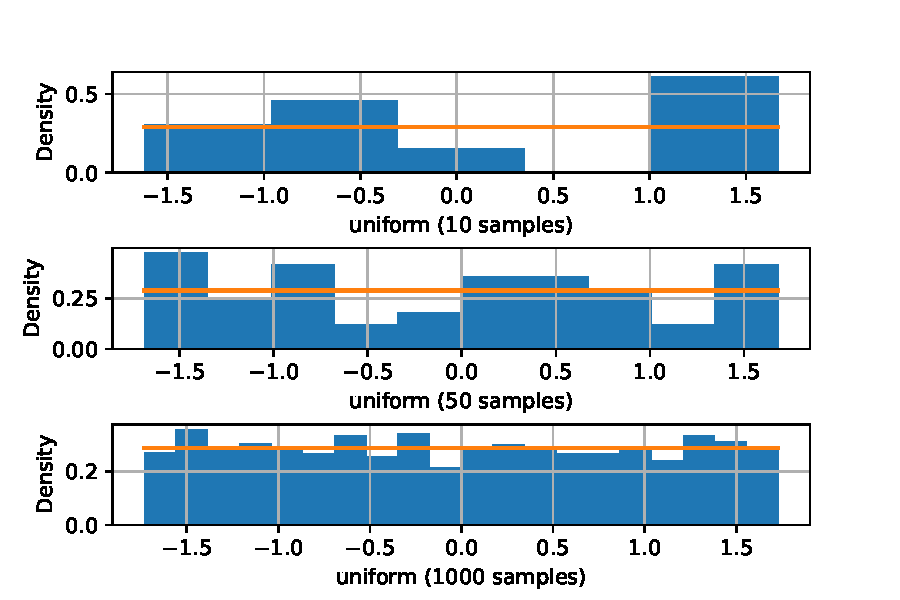
\includegraphics[width = 16 cm]{src_lab_1/uniform}
            \caption{Равномерное Распределение~\eqref{eq:uniform}}
            \label{fig:uniform}
        \end{figure}

    	\subsection{Характеристики положения и рассеяния}
	\noindent Как было проведено округление:\\
В оценке $x=E  \pm D$ вариации подлежит первая цифра после точки. В данном случае $x=0.0 \pm 0.1k$,  $k$ - зависит от доверительной вероятности и вида распределения (рассматривается в дальнейшем цикле лабораторных работ). Округление сделано для  $k=1$.

	        \begin{table}[H]
            \centering
            \begin{tabular}{|c|c|c|c|c|c|}
                \hline
                 &$\overline{x}$&$med\ x$&$z_R$&$z_Q$&$z_{tr}$ \\ \hline
$E\left(z\right)$&0.0125&0.0038&0.0264&0.3263&0.2863\\ \hline
$D\left(z\right)$&0.0961&0.1256&0.1905&0.1166&0.1049\\ \hline
$E + \sqrt{D}$&0.3224&0.3582&0.4629&0.6678&0.6101\\ \hline
$E - \sqrt{D}$&-0.2975&-0.3506&-0.4101&-0.0152&-0.0375\\ \hline
\widehat{E}(z)&-&0.12&0.1&-&-\\ \hline

            \end{tabular}
            \caption{Нормальное распределение 10 элементов}
            \label{tab:norm_10}
        \end{table}

        \begin{table}[H]
            \centering
            \begin{tabular}{|c|c|c|c|c|c|}
                \hline
                 &$\overline{x}$&$med\ x$&$z_R$&$z_Q$&$z_{tr}$ \\ \hline
$E\left(z\right)$&-0.0002&0.0014&-0.0073&0.0168&0.0144\\ \hline
$D\left(z\right)$&0.0099&0.0156&0.0995&0.0122&0.0115\\ \hline

            \end{tabular}
            \caption{Нормальное распределение 100 элементов}
            \label{tab:norm_100}
        \end{table}

         \begin{table}[H]
            \centering
            \begin{tabular}{|c|c|c|c|c|c|}
                \hline
                 &$\overline{x}$&$med\ x$&$z_R$&$z_Q$&$z_{tr}$ \\ \hline
$E\left(z\right)$&-0.0003&-0.0008&-0.0041&0.0009&0.0022\\ \hline
$D\left(z\right)$&0.001&0.0016&0.0593&0.0012&0.0012\\ \hline
$E + \sqrt{D}$&0.0306&0.0388&0.2394&0.0361&0.0366\\ \hline
$E - \sqrt{D}$&-0.0312&-0.0404&-0.2477&-0.0344&-0.0321\\ \hline
\widehat{E}(z)&0.0&0.0&0.0&0.0&0.0\\ \hline

            \end{tabular}
            \caption{Нормальное распределение 1000 элементов}
            \label{tab:norm_1000}
        \end{table}

        \begin{table}[H]
            \centering
            \begin{tabular}{|c|c|c|c|c|c|}
                \hline
                 &$\overline{x}$&$med\ x$&$z_R$&$z_Q$&$z_{tr}$ \\ \hline
$E\left(z\right)$&0.7254&0.0313&3.1868&1.4041&0.2585\\ \hline
$D\left(z\right)$&194.3172&0.3554&4604.129&9.3915&0.3452\\ \hline

            \end{tabular}
            \caption{Распределение Коши 10 элементов}
            \label{tab:cauchy_10}
        \end{table}

        \begin{table}[H]
            \centering
            \begin{tabular}{|c|c|c|c|c|c|}
                \hline
                 &$\overline{x}$&$med\ x$&$z_R$&$z_Q$&$z_{tr}$ \\ \hline
$E\left(z\right)$&0.6253&-0.0102&32.4295&0.0233&0.0094\\ \hline
$D\left(z\right)$&447.9305&0.0246&1107035.055&0.0534&0.0262\\ \hline

            \end{tabular}
            \caption{Распределение Коши 100 элементов}
            \label{tab:cauchy_100}
        \end{table}

        \begin{table}[H]
            \centering
            \begin{tabular}{|c|c|c|c|c|c|}
                \hline
                 &$\overline{x}$&$med\ x$&$z_R$&$z_Q$&$z_{tr}$ \\ \hline
$E\left(z\right)$&-0.2614&0.0&-113.7389&-0.0003&0.0005\\ \hline
$D\left(z\right)$&131.9924&0.0023&29640377.6809&0.0048&0.0023\\ \hline

            \end{tabular}
            \caption{Распределение Коши 1000 элементов}
            \label{tab:cauchy_1000}
        \end{table}

        \begin{table}[H]
            \centering
            \begin{tabular}{|c|c|c|c|c|c|}
                \hline
                 &$\overline{x}$&$med\ x$&$z_R$&$z_Q$&$z_{tr}$ \\ \hline
$E\left(z\right)$&-0.0017&0.0003&0.0012&0.4187&0.3298\\ \hline
$D\left(z\right)$&0.1954&0.1365&0.8186&0.2293&0.1584\\ \hline
$E + \sqrt{D}$&0.4404&0.3699&0.906&0.8975&0.7277\\ \hline
$E - \sqrt{D}$&-0.4437&-0.3692&-0.9035&-0.0602&-0.0682\\ \hline
\widehat{E}(z)&0.19&0.136&0.81&-&-\\ \hline

            \end{tabular}
            \caption{Распределение Лапласа 10 элементов}
            \label{tab:laplace_10}
        \end{table}

        \begin{table}[H]
            \centering
            \begin{tabular}{|c|c|c|c|c|c|}
                \hline
                 &$\overline{x}$&$med\ x$&$z_R$&$z_Q$&$z_{tr}$ \\ \hline
$E\left(z\right)$&-0.0035&-0.0041&0.0086&0.0184&0.0261\\ \hline
$D\left(z\right)$&0.02&0.0121&0.7719&0.0193&0.0128\\ \hline
$E + \sqrt{D}$&0.1377&0.1059&0.8872&0.1573&0.1394\\ \hline
$E - \sqrt{D}$&-0.1448&-0.1141&-0.87&-0.1205&-0.0871\\ \hline
\widehat{E}(z)&0.0&0.0&0.7&0.0&-\\ \hline

            \end{tabular}
            \caption{Распределение Лапласа 100 элементов}
            \label{tab:laplace_100}
        \end{table}

        \begin{table}[H]
            \centering
            \begin{tabular}{|c|c|c|c|c|c|}
                \hline
                 &$\overline{x}$&$med\ x$&$z_R$&$z_Q$&$z_{tr}$ \\ \hline
$E\left(z\right)$&0.0023&0.0017&-0.0219&0.0039&0.0035\\ \hline
$D\left(z\right)$&0.0018&0.001&0.8525&0.0018&0.0011\\ \hline

            \end{tabular}
            \caption{Распределение Лапласа 1000 элементов}
            \label{tab:laplace_1000}
        \end{table}

        \begin{table}[H]
            \centering
            \begin{tabular}{|c|c|c|c|c|c|}
                \hline
                 &$\overline{x}$&$med\ x$&$z_R$&$z_Q$&$z_{tr}$ \\ \hline
$E\left(z\right)$&9.9637&9.834&10.2755&10.895&8.5507\\ \hline
$D\left(z\right)$&1.0235&1.4704&1.9523&1.368&0.8573\\ \hline

            \end{tabular}
            \caption{Распределение Пуассона 10 элементов}
            \label{tab:poisson_10}
        \end{table}

        \begin{table}[H]
            \centering
            \begin{tabular}{|c|c|c|c|c|c|}
                \hline
                 &$\overline{x}$&$med\ x$&$z_R$&$z_Q$&$z_{tr}$ \\ \hline
$E\left(z\right)$&9.997&9.837&10.977&9.9555&9.6981\\ \hline
$D\left(z\right)$&0.0971&0.2039&1.0005&0.1503&0.1158\\ \hline

            \end{tabular}
            \caption{Распределение Пуассона 100 элементов}
            \label{tab:poisson_100}
        \end{table}

        \begin{table}[H]
            \centering
            \begin{tabular}{|c|c|c|c|c|c|}
                \hline
                 &$\overline{x}$&$med\ x$&$z_R$&$z_Q$&$z_{tr}$ \\ \hline
$E\left(z\right)$&10.0033&9.996&11.634&9.998&9.8458\\ \hline
$D\left(z\right)$&0.0098&0.004&0.6395&0.0015&0.0108\\ \hline

            \end{tabular}
            \caption{Распределение Пуассона 1000 элементов}
            \label{tab:poisson_1000}
        \end{table}

        \begin{table}[H]
            \centering
            \begin{tabular}{|c|c|c|c|c|c|}
                \hline
                 &$\overline{x}$&$med\ x$&$z_R$&$z_Q$&$z_{tr}$ \\ \hline
$E\left(z\right)$&-0.0178&-0.0205&-0.0079&0.2859&0.1164\\ \hline
$D\left(z\right)$&0.0985&0.2222&0.0469&0.1304&0.1205\\ \hline

            \end{tabular}
            \caption{Равномерное распределение 10 элементов}
            \label{tab:uniform_10}
        \end{table}

        \begin{table}[H]
            \centering
            \begin{tabular}{|c|c|c|c|c|c|}
                \hline
                 &$\overline{x}$&$med\ x$&$z_R$&$z_Q$&$z_{tr}$ \\ \hline
$E\left(z\right)$&-0.0061&-0.0104&-0.0012&0.0113&0.0085\\ \hline
$D\left(z\right)$&0.0092&0.0279&0.0006&0.0141&0.0176\\ \hline

            \end{tabular}
            \caption{Равномерное распределение 100 элементов}
            \label{tab:uniform_100}
        \end{table}

        \begin{table}[H]
            \centering
            \begin{tabular}{|c|c|c|c|c|c|}
                \hline
                 &$\overline{x}$&$med\ x$&$z_R$&$z_Q$&$z_{tr}$ \\ \hline
$E\left(z\right)$&0.002&0.0028&0.0&0.0038&0.0048\\ \hline
$D\left(z\right)$&0.001&0.0029&0.0&0.0015&0.0019\\ \hline

            \end{tabular}
            \caption{Равномерное распределение 1000 элементов}
            \label{tab:uniform_1000}
        \end{table}

    \subsection{Боксплот Тьюки}
\begin{figure}[H]
\center{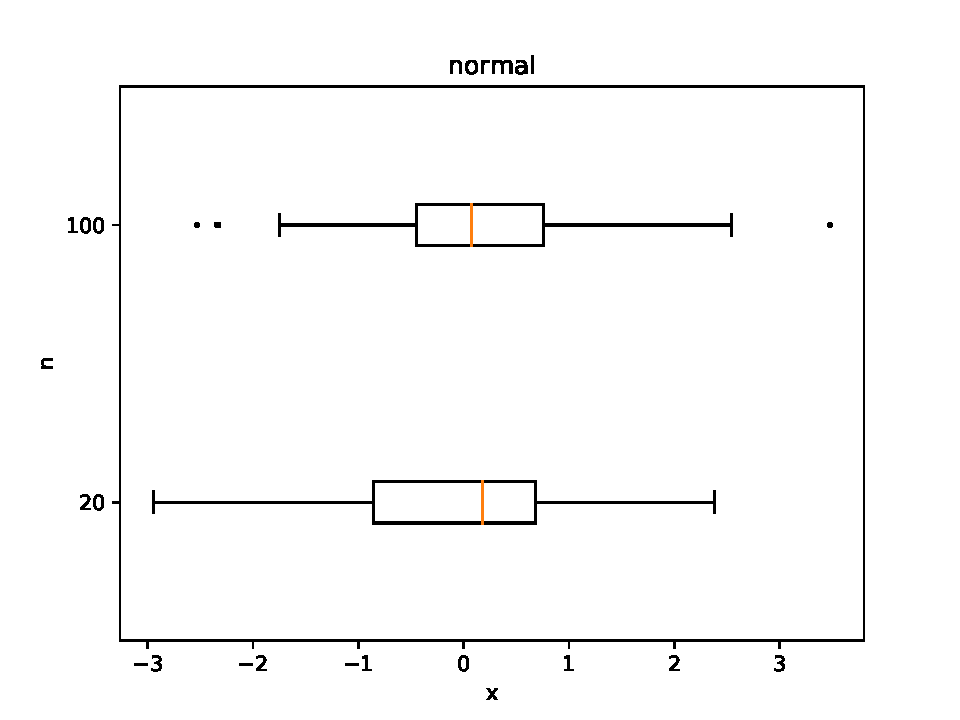
\includegraphics[scale=0.75]{src_lab_3/normal}}
\label{fig:normal}
\caption{Нормальное распределение}
\end{figure}

\begin{figure}[H]
\center{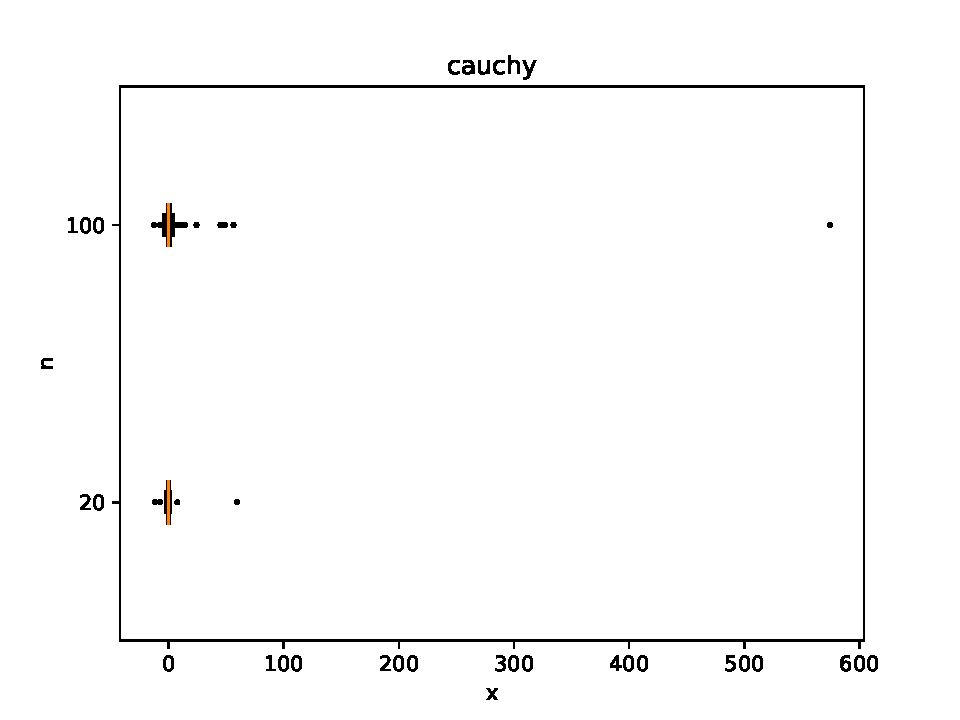
\includegraphics[scale=0.75]{src_lab_3/cauchy}}
\label{fig:cauchy}
\caption{распределение Коши}
\end{figure}

\begin{figure}[H]
\center{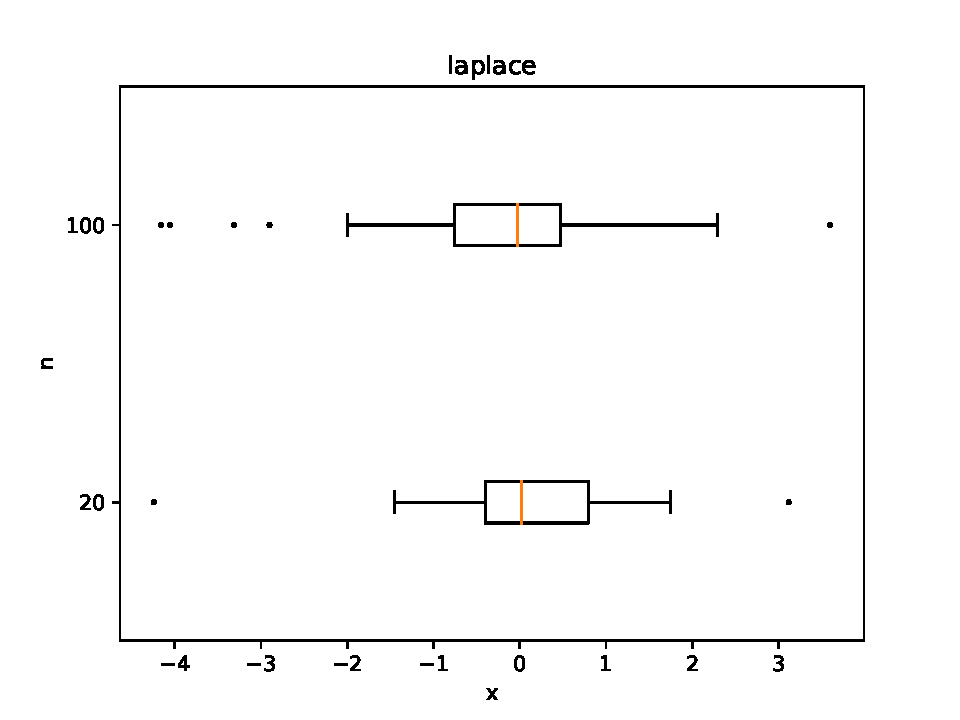
\includegraphics[scale=0.75]{src_lab_3/laplace}}
\label{fig:laplace}
\caption{распределение Лапласа}
\end{figure}

\begin{figure}[H]
\center{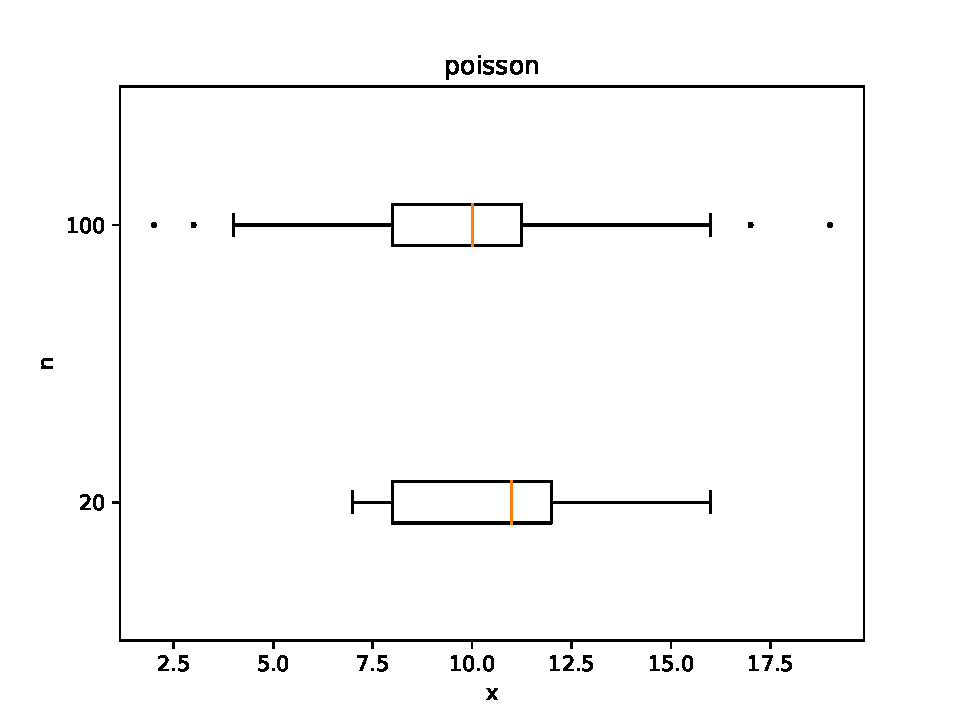
\includegraphics[scale=0.75]{src_lab_3/poisson}}
\label{fig:poisson}
\caption{распределение Пуассона}
\end{figure}

\begin{figure}[H]
\center{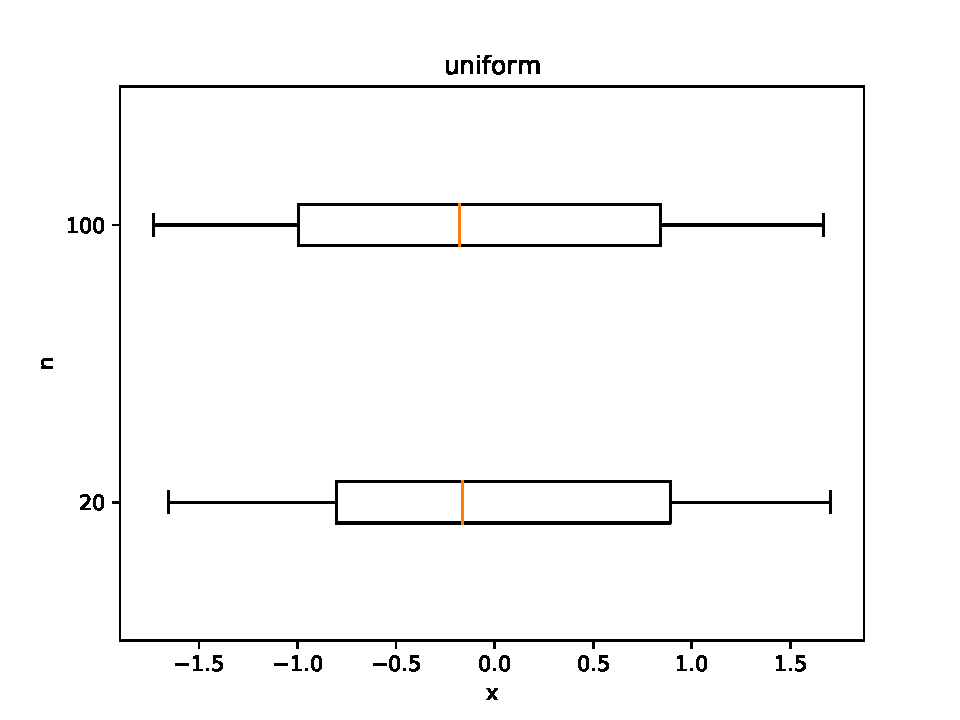
\includegraphics[scale=0.75]{src_lab_3/uniform}}
\label{fig:uniform}
\caption{равномерное распределение}
\end{figure}

\subsection{Доля выбросов}
\begin{table}[H]
            \centering
            \begin{tabular}{|c|c|c|}
                \hline
                sample size&20&100\\ \hline
normal&0.024&0.01\\ \hline
cauchy&0.155&0.157\\ \hline
laplace&0.076&0.064\\ \hline
poisson&0.025&0.011\\ \hline
uniform&0.003&0.0\\ \hline

            \end{tabular}
            \caption{Доля выбросов}
            \label{tab:experimental_anomaly}
            \end{table}


\subsection{Теоретическая вероятность выбросов}
\begin{table}[H]
            \centering
            \begin{tabular}{|c|c|c|c|c|c|}
                \hline
                &$Q^{T}_{1}$&$Q^{T}_{3}$&$X^{T}_{1}$&$X^{T}_{2}$&$P^{T}_{B}$\\ \hline
normal&-0.674&0.674&-2.698&2.698&0.007\\ \hline
cauchy&-1.0&1.0&-4.0&4.0&0.156\\ \hline
laplace&-0.49&0.49&-1.961&1.961&0.062\\ \hline
poisson&8.0&12.0&2.0&18.0&0.008\\ \hline
uniform&-0.866&0.866&-3.464&3.464&0.0\\ \hline

            \end{tabular}
            \caption{Теоретическая вероятность выбросов}
            \label{tab:theoretical_anomaly}
            \end{table}

	
	
\subsection{Эмпирическая функция распределения}
	\begin{figure}[H]
	\centering
	\centering
	{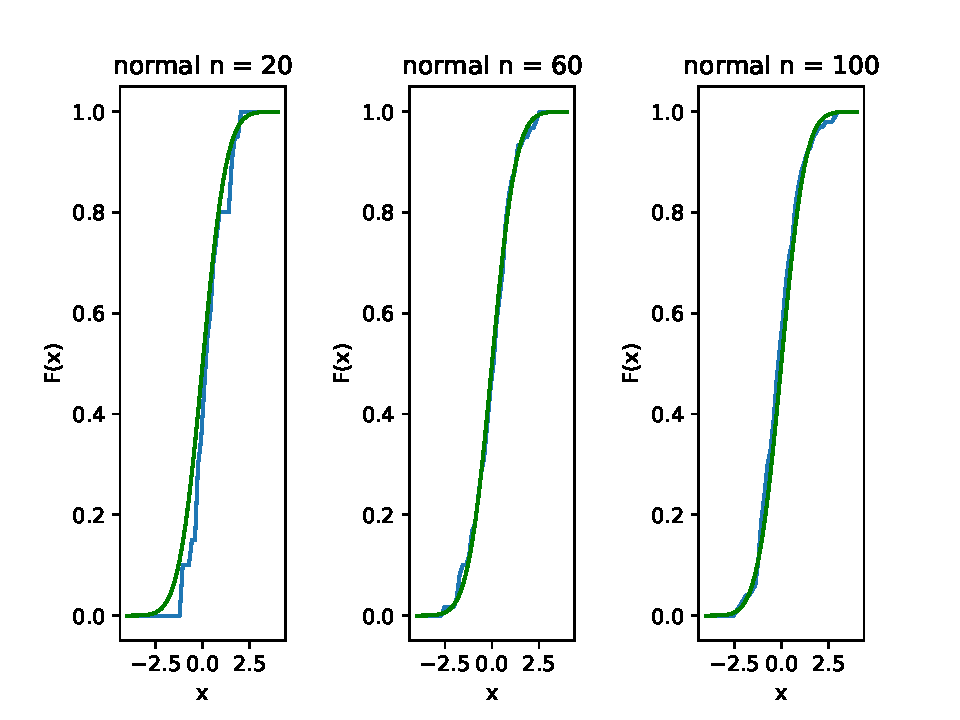
\includegraphics[scale=0.5]{src_lab_4/emperical_fun_normal}}
		\caption{Нормальное распределение}
		\label{fig:normal}
	\end{figure}

\begin{figure}[H]
	\centering
	{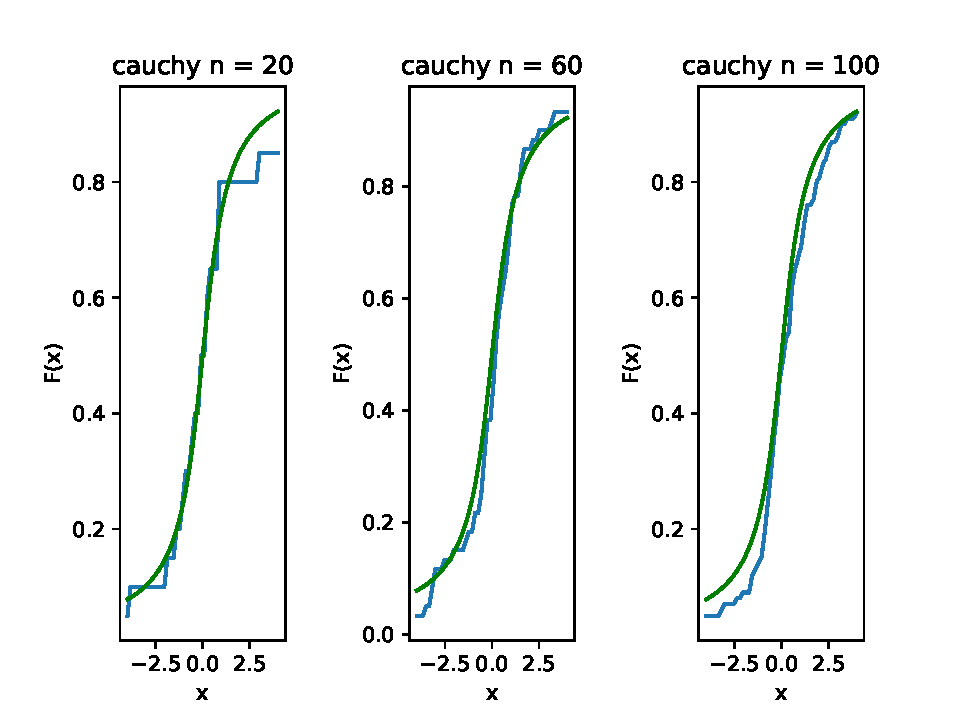
\includegraphics[scale=0.5]{src_lab_4/emperical_fun_cauchy}}
		\caption{Распределение Коши}
		\label{fig:cauchy}
	\end{figure}

\begin{figure}[H]
	\centering
	{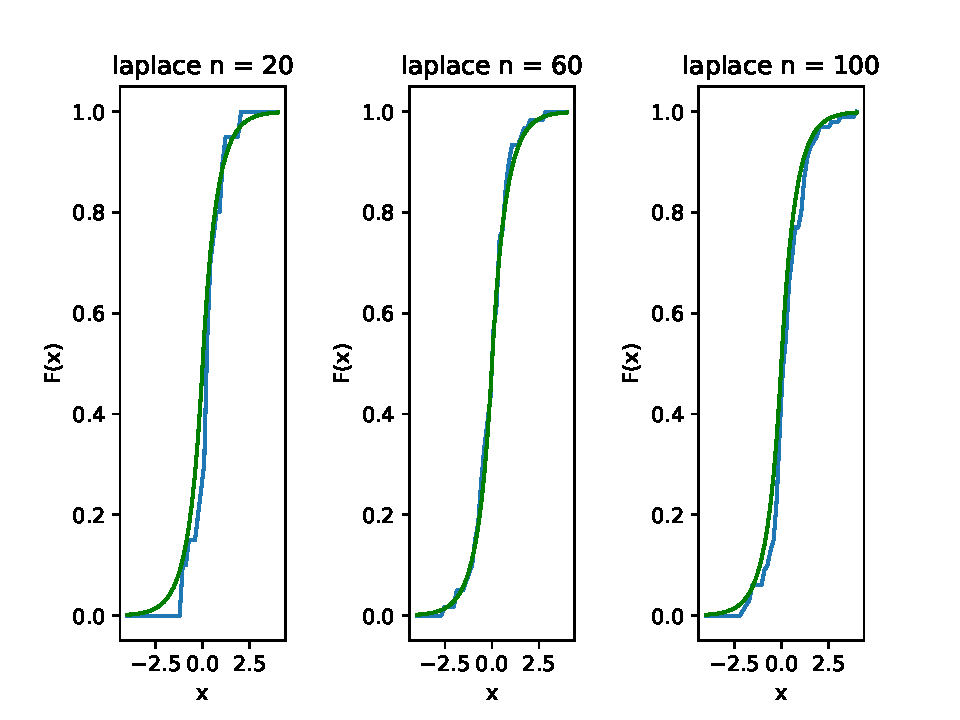
\includegraphics[scale=0.5]{src_lab_4/emperical_fun_laplace}}
		\caption{Распределение Лапласа}
		\label{fig:laplace}
	\end{figure}

\begin{figure}[H]
	\centering
	{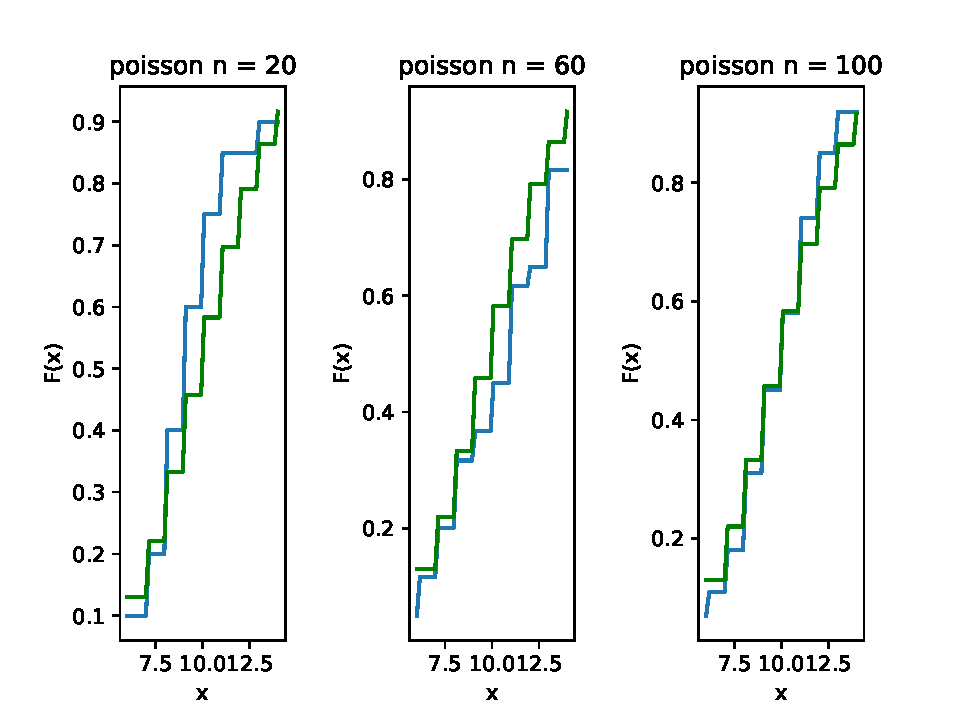
\includegraphics[scale=0.5]{src_lab_4/emperical_fun_poisson}}
		\caption{Распределение Пуассона}
		\label{fig:posson}
	\end{figure}

\begin{figure}[H]
	\centering
	{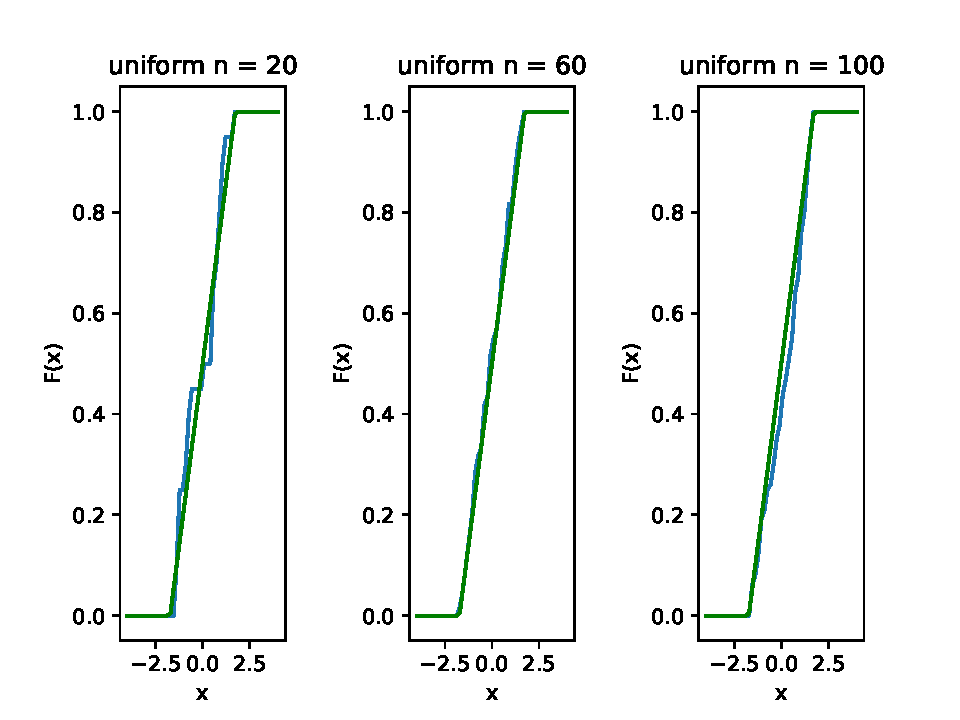
\includegraphics[scale=0.5]{src_lab_4/emperical_fun_uniform}}
		\caption{Равномерное распределение}
		\label{fig:uniform}
	\end{figure}

\subsection{Ядерные оценки плотности распределения}
\begin{figure}[H]
	\centering
	{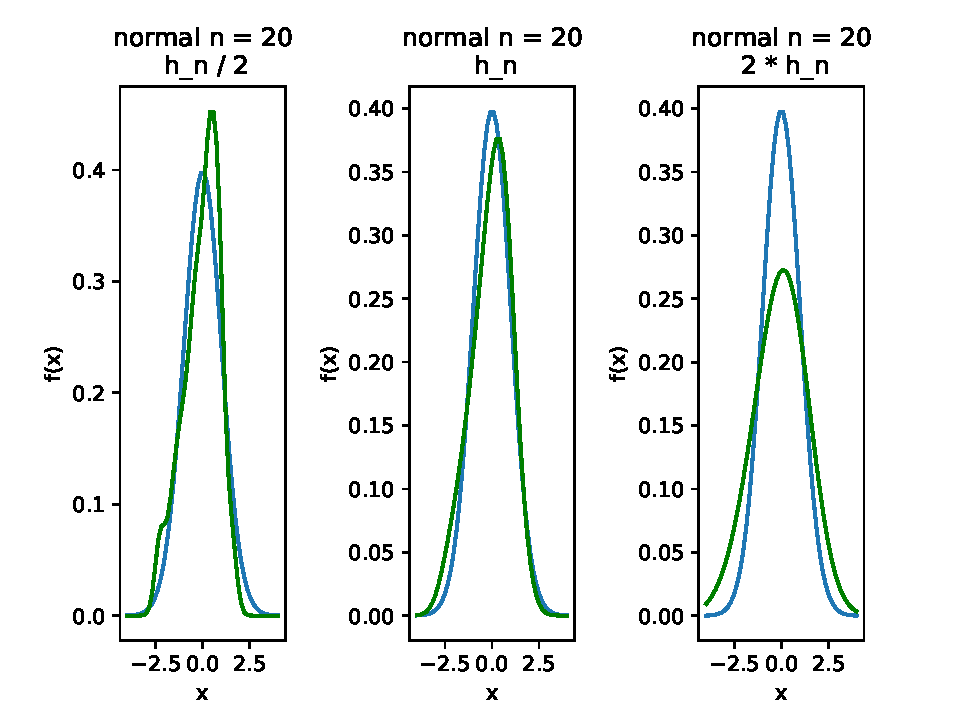
\includegraphics[scale=0.5]{src_lab_4/kde_20_normal}}
		\caption{Нормальное распределение, $n=20$}
		\label{fig:kde_normal_20}
	\end{figure}

\begin{figure}[H]
	\centering
	{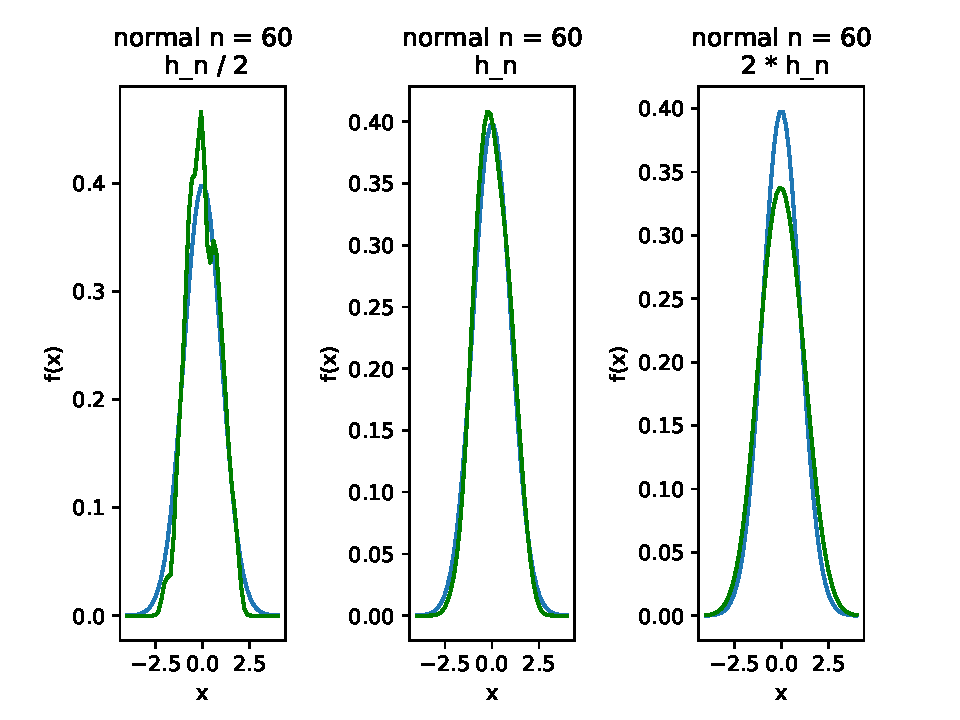
\includegraphics[scale=0.5]{src_lab_4/kde_60_normal}}
		\caption{Нормальное распределение, $n=60$}
		\label{fig:kde_normal_60}
	\end{figure}

\begin{figure}[H]
	\centering
	{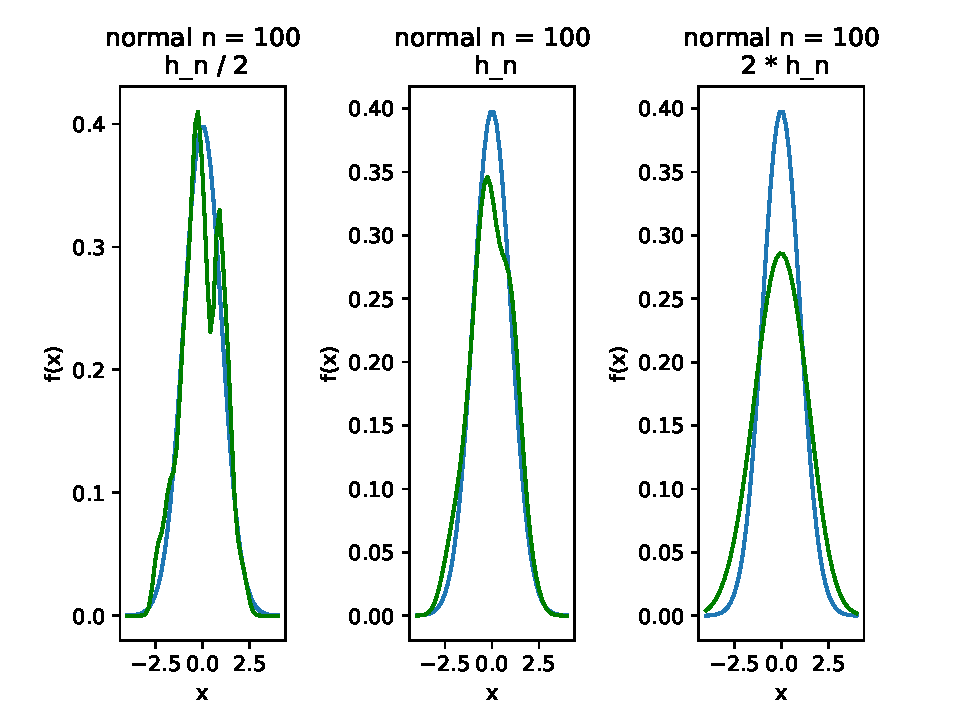
\includegraphics[scale=0.5]{src_lab_4/kde_100_normal}}
		\caption{Нормальное распределение, $n=100$}
		\label{fig:kde_normal_100}
	\end{figure}

\begin{figure}[H]
	\centering
	{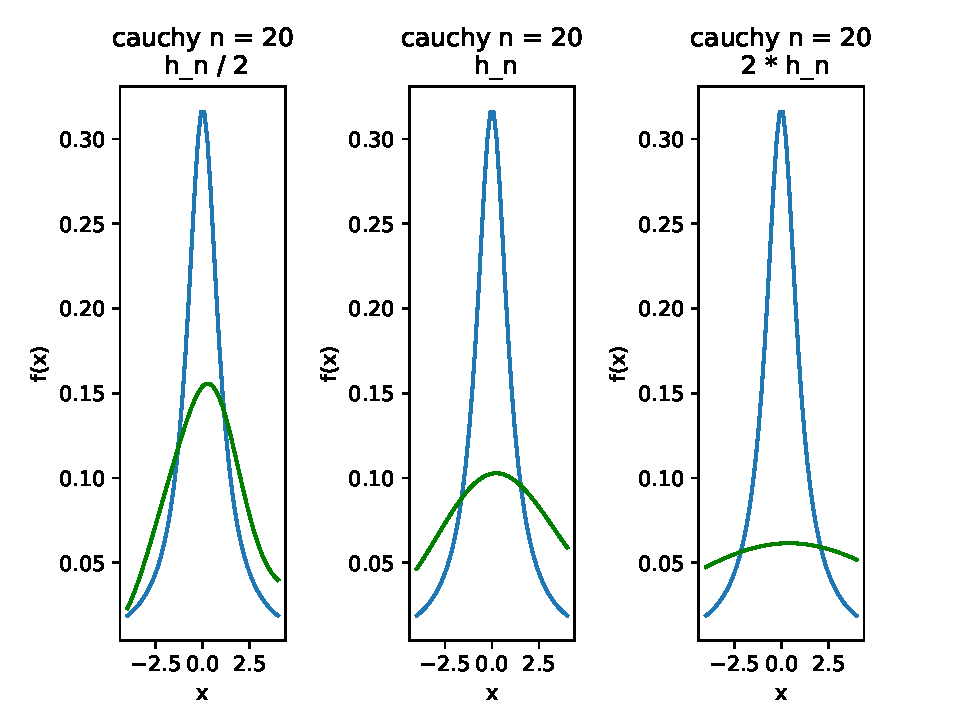
\includegraphics[scale=0.5]{src_lab_4/kde_20_cauchy}}
		\caption{Распределение Коши, $n=20$}
		\label{fig:kde_cauchy_20}
	\end{figure}

\begin{figure}[H]
	\centering
	{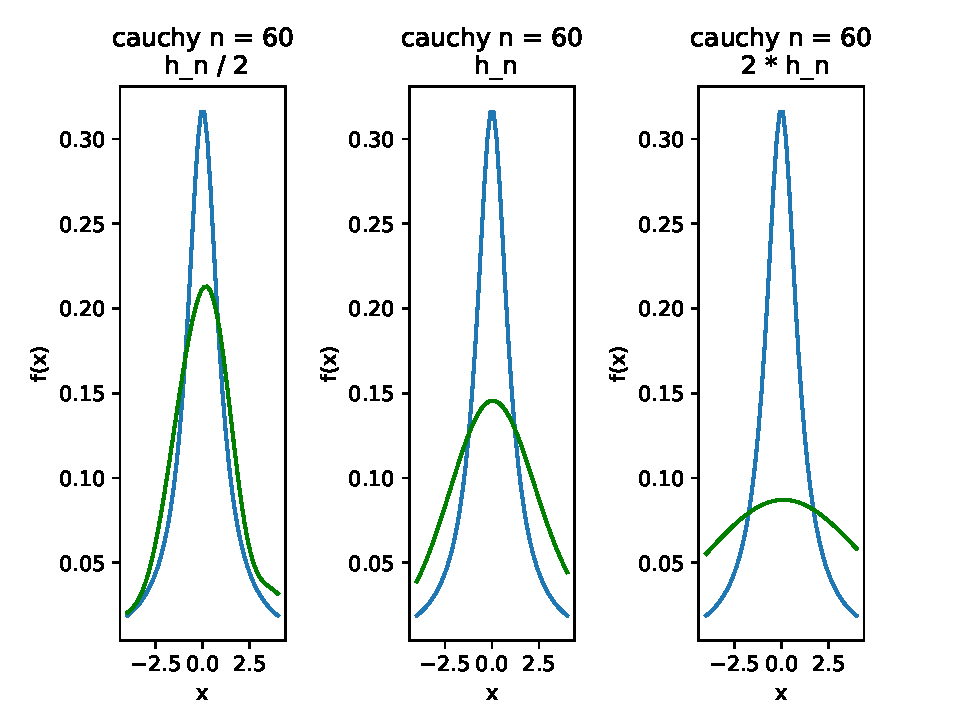
\includegraphics[scale=0.5]{src_lab_4/kde_60_cauchy}}
		\caption{Распределение Коши, $n=60$}
		\label{fig:kde_cauchy_60}
	\end{figure}

\begin{figure}[H]
	\centering
	{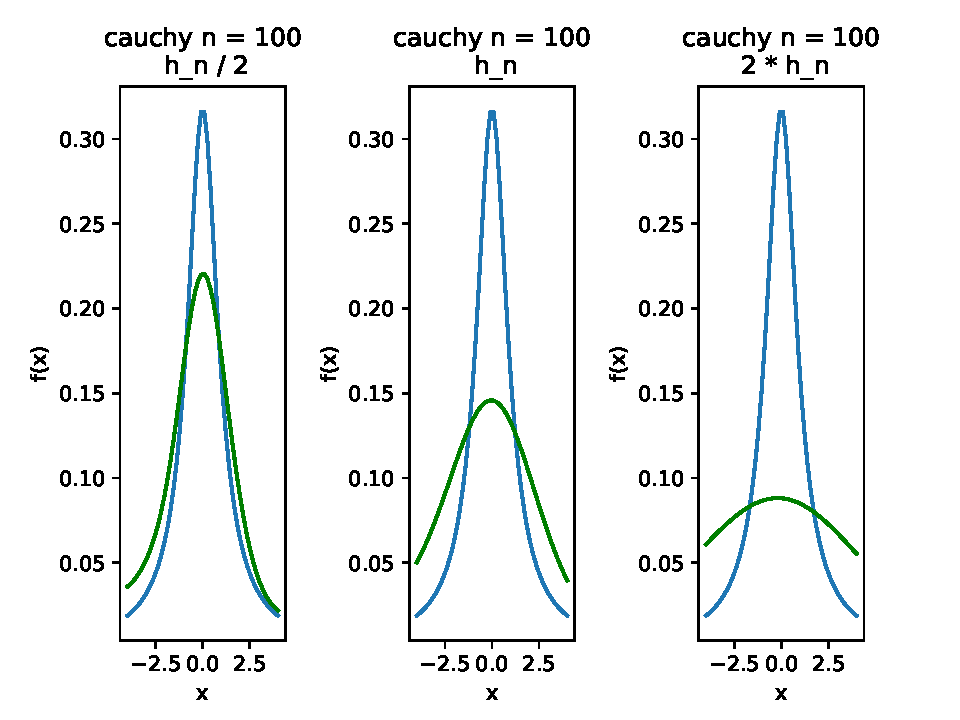
\includegraphics[scale=0.5]{src_lab_4/kde_100_cauchy}}
		\caption{Hаспределение Коши, $n=100$}
		\label{fig:kde_cauchy_100}
	\end{figure}

\begin{figure}[H]
	\centering
	{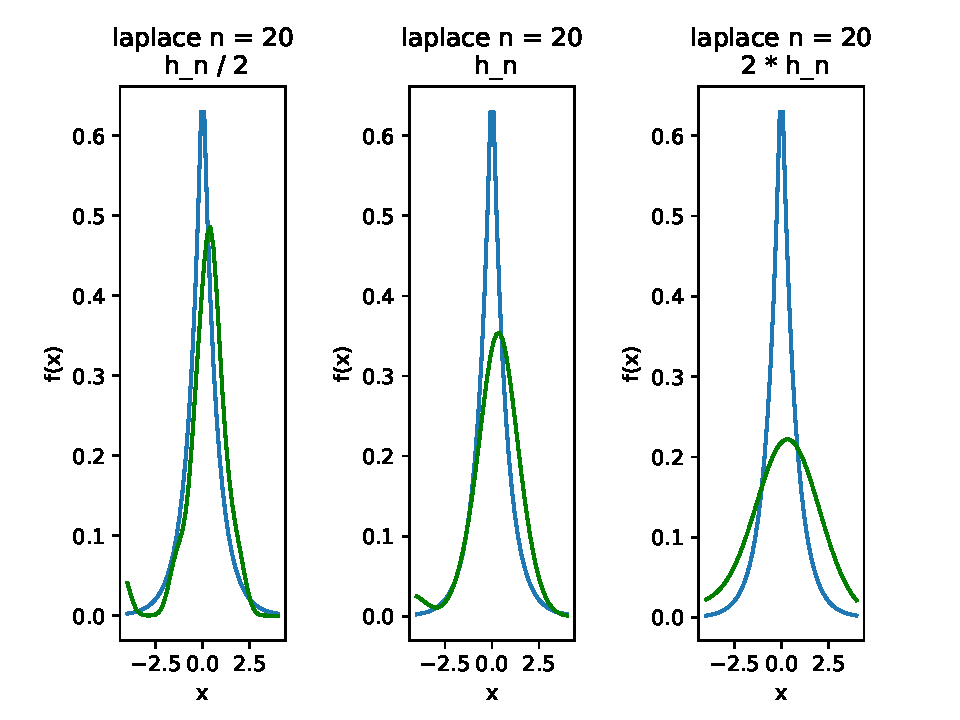
\includegraphics[scale=0.5]{src_lab_4/kde_20_laplace}}
		\caption{Распределение Лапласа, $n=20$}
		\label{fig:kde_laplace_20}
	\end{figure}

\begin{figure}[H]
	\centering
	{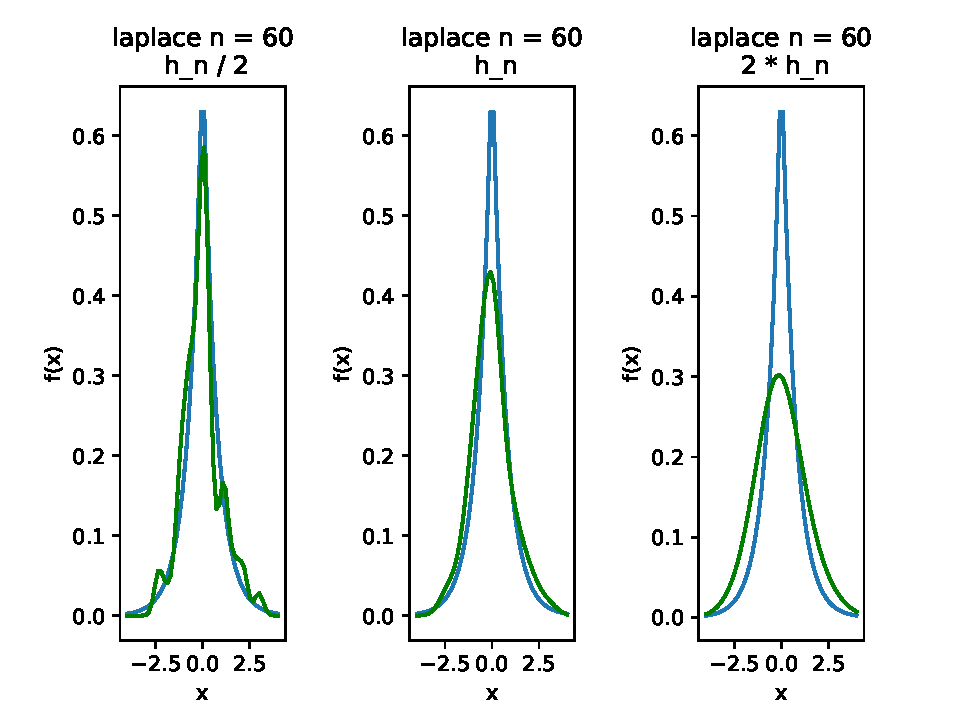
\includegraphics[scale=0.5]{src_lab_4/kde_60_laplace}}
		\caption{Распределение Лапласа, $n=60$}
		\label{fig:kde_laplace_60}
	\end{figure}

\begin{figure}[H]
	\centering
	{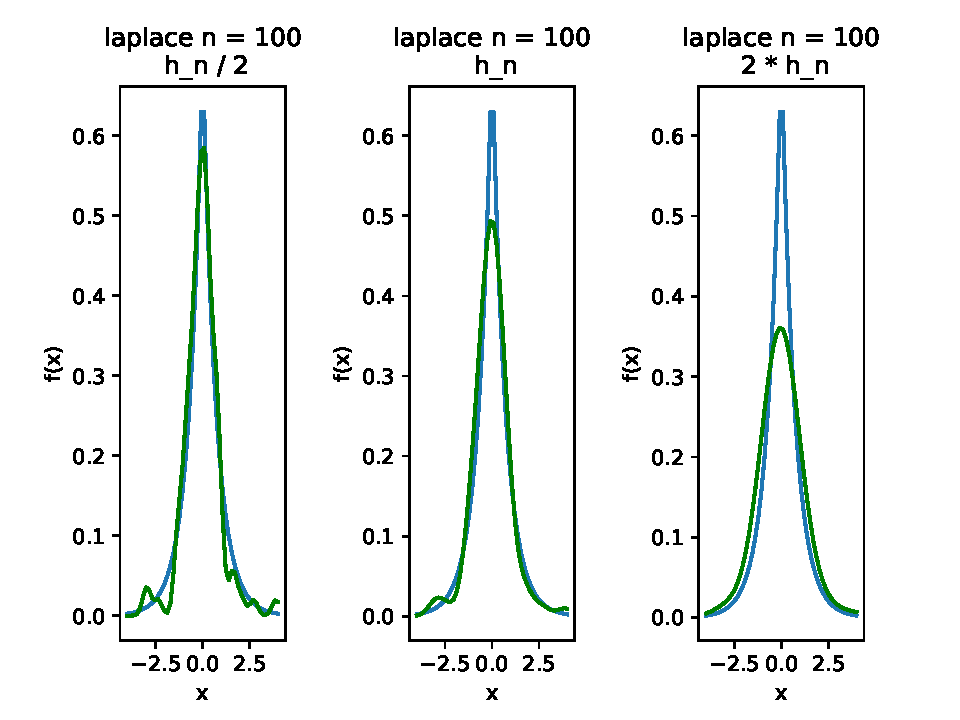
\includegraphics[scale=0.5]{src_lab_4/kde_100_laplace}}
		\caption{Распределение Лапласа, $n=100$}
		\label{fig:kde_laplace_100}
	\end{figure}

\begin{figure}[H]
	\centering
	{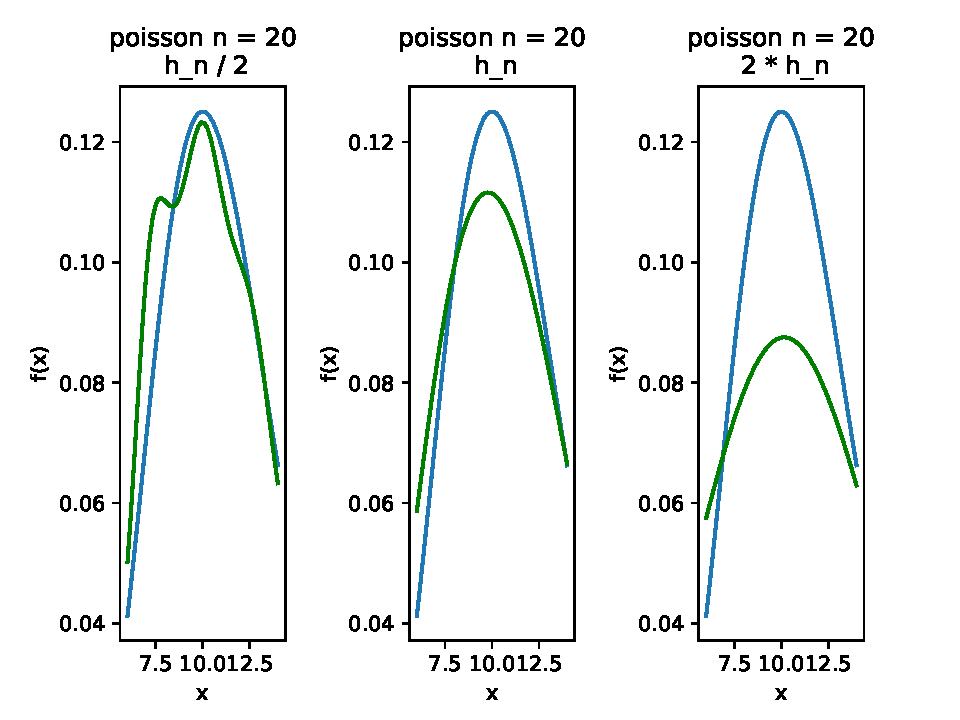
\includegraphics[scale=0.5]{src_lab_4/kde_20_poisson}}
		\caption{Распределение Пуассона, $n=20$}
		\label{fig:kde_poisson_20}
	\end{figure}

\begin{figure}[H]
	\centering
	{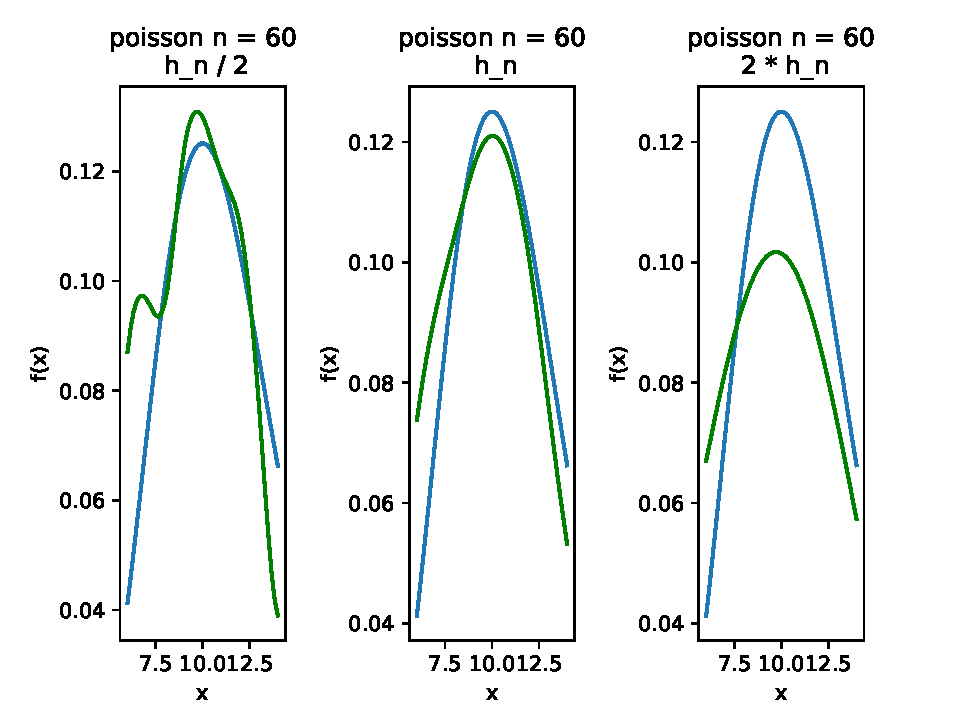
\includegraphics[scale=0.5]{src_lab_4/kde_60_poisson}}
		\caption{Распределение Пуассона, $n=60$}
		\label{fig:kde_poisson_60}
	\end{figure}

\begin{figure}[H]
	\centering
	{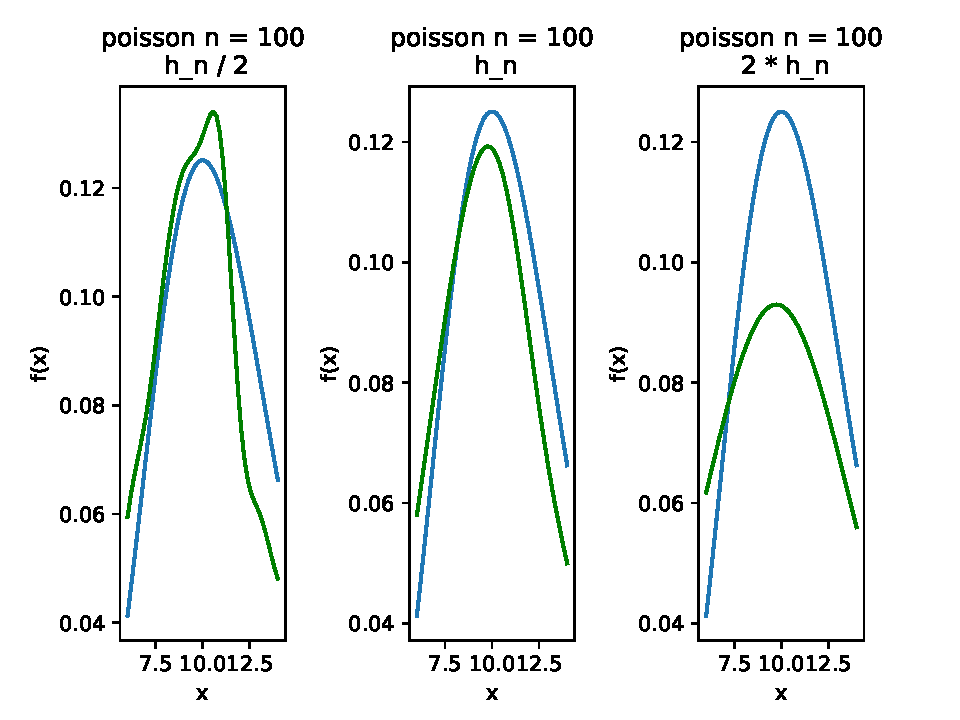
\includegraphics[scale=0.5]{src_lab_4/kde_100_poisson}}
		\caption{Распределение Пуассона, $n=100$}
		\label{fig:kde_poisson_100}
	\end{figure}

\begin{figure}[H]
	\centering
	{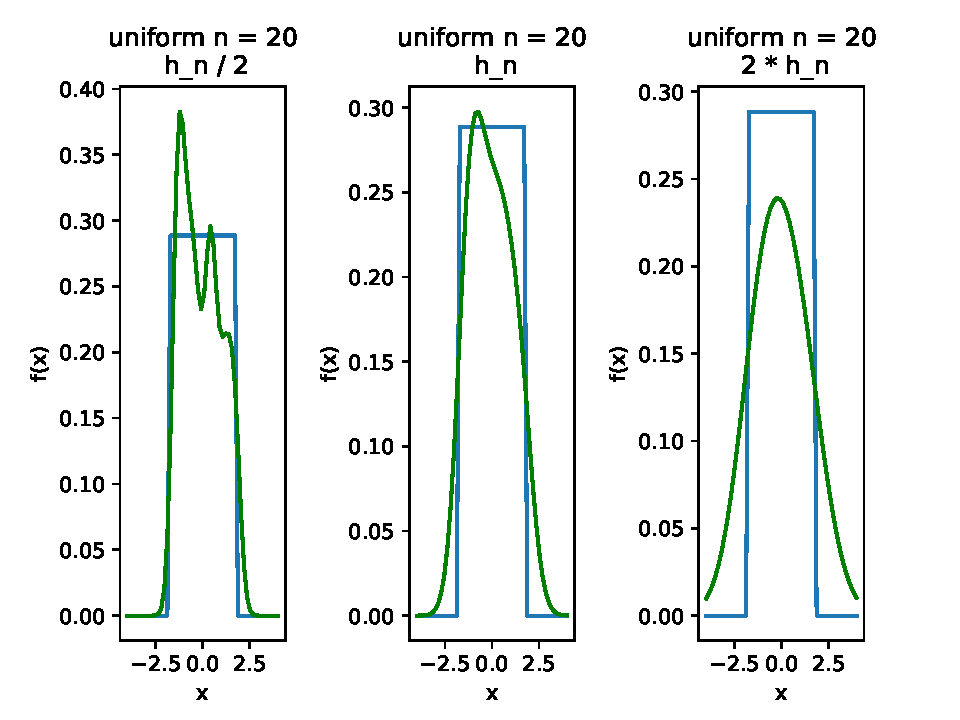
\includegraphics[scale=0.5]{src_lab_4/kde_20_uniform}}
		\caption{Равномерное распределение, $n=20$}
		\label{fig:kde_uniform_20}
	\end{figure}

\begin{figure}[H]
	\centering
	{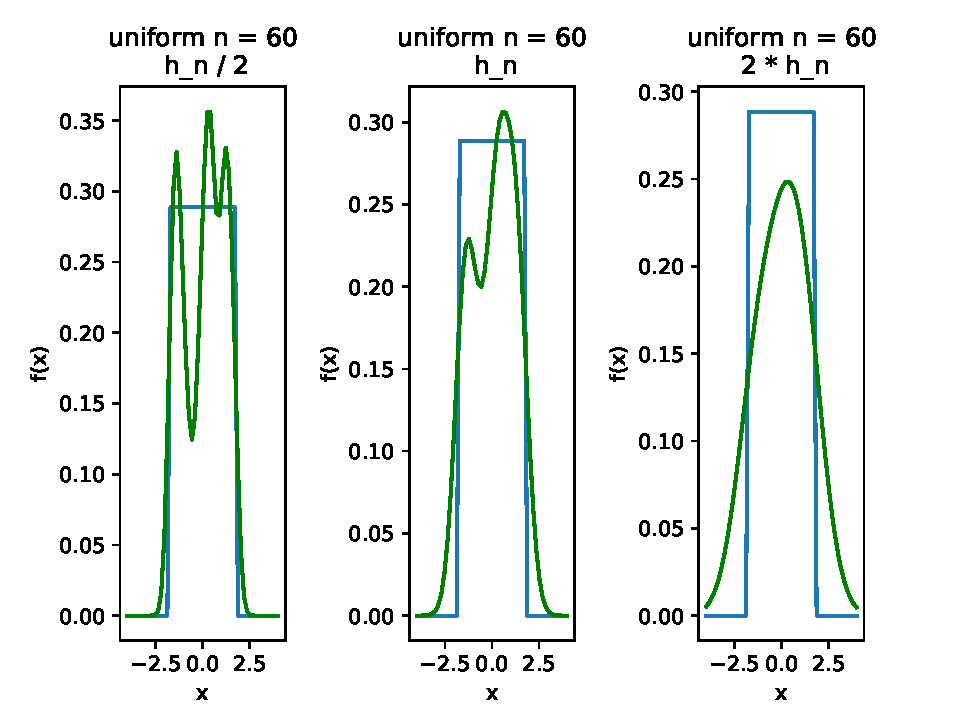
\includegraphics[scale=0.5]{src_lab_4/kde_60_uniform}}
		\caption{Равномерное распределение, $n=60$}
		\label{fig:kde_uniform_60}
	\end{figure}

\begin{figure}[H]
	\centering
	{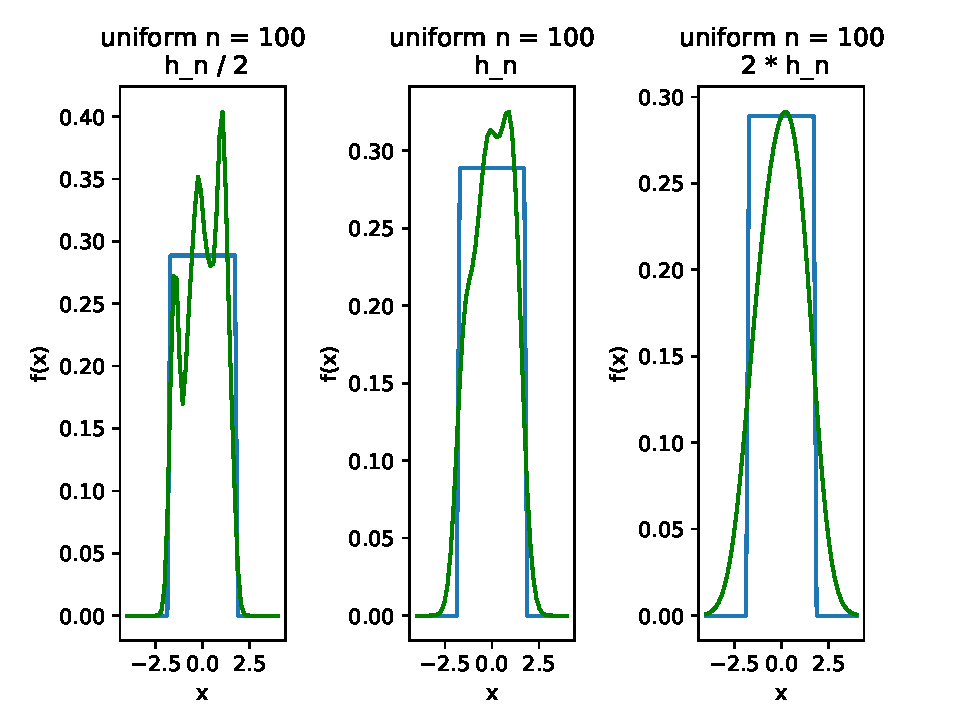
\includegraphics[scale=0.5]{src_lab_4/kde_100_uniform}}
		\caption{Равномерное распределение, $n=100$}
		\label{fig:kde_uniform_100}
	\end{figure}
\section{Обсуждение}
    \subsection{Гистограмма и график плотности распределения}
        Видно, что во всех рассмотренных случаях при увеличении размера выборки гистограмма приближается к графику функции плотности вероятности закона, по которому распределены элементы.
        При малом размере выборки невозможно понять по какому распределению генерировалась выборка так как все гистограммы похожи друг на друга.
    \subsection{Характеристики положения и рассеяния}
        Можно заметить, что дисперсия характеристик рассеяния для распределения Коши является аномально болишим по сравнению с другими распределениями.
        Даже при увиличении размера выборки ситуация не меняется. Это можно обяснить выбросами, которые наблюдались в результатах предыдущей работы.
    \subsection{Доля и теоретическая вероятность выбросов}
        В данной работе видно, что боксплоты Тьюки удобны для взуального представления важных
        характеристик выборки. Из них можно делать выводы относительно
        вида распределения, которому подчиняется выборка.

        Данные в таблице говорят о том, что чем выше размер выборки, тем ближе доля выбросов к теоретической оценке. У распределения коши наблюдается самая высокая доля выбросов, в то время как в равномерном распределении доля выбросов близка к 0.

    \subsection{Эмпирическая функция и ядерные оценки плотности распределения}
        На представленных графиках видно, что эмпирическая функция распределения тем лучше приближает функцию распределения заказа, чем больший объем выборки мы берём. Наибольшие отклонения наблюдаются для распределения Пуассона и равномерного распределения.


        По иллюстрациям, относящимся к ядерным оценкам плотности вероятности можно увидеть, что снова качество приближения увеличивается с увеличением размеров выборки. При этом выбор оптимального параметра h отличается для разных распределений. Например, для распределения Лапласа лучшие результаты даёт $h_n=0.5$

        Чем больше числовой коэффициент при параметре сглаживания $h_n$, тем менньшее количество раз происходит чередование знака производной аппроксимирующей функции на рассматриваемом промежуткем. При выборе коэффициента равного 2 мы приходим к цнимодальной функции и полученные приближения перестают описывать особенности распределения, так что становится невозможно сказать что-то о законе распредления случайной величины.



\section{Приложение}

С кодом работ и отчета можно ознакомиться по ссылке:\;\url{https://github.com/sqrtyyy/MathStat/tree/master}
\end{document}